\chapter{Specifikacija programske potpore}
		
	\section{Funkcionalni zahtjevi}
		
			
			\noindent \textbf{Dionici:}
			
			\begin{packed_enum}
				
				\item Udruge za životinje
				\item Građani
				\begin{packed_enum}
				    \item registrirani korisnici
				    \item javni posjetitelji
				\end{packed_enum}
				\item Administrator
				\item Razvojni tim
				
			\end{packed_enum}
			
			\noindent \textbf{Aktori i njihovi funkcionalni zahtjevi:}
			
			
			\begin{packed_enum}
				\item  \underbar{Neregistrirani/neprijavljeni korisnik (inicijator) može:}
				
				\begin{packed_enum}
					
					\item pregledati listu svih registriranih udruga
					
					\item pregledati svaku pojedinu registriranu udrugu i dobiti prikaz općih informacija (ime udruge, slika, OIB, e-mail, adresa)
					
					\item pregledati pse pojedine udruge i dobiti prikaz općih  informacija (ime, slika, opis, vrsta šetnje, pasmina, lokacija, raspoloživost)
					
					\item pogledati rang listu registriranih šetača s javnim profilom prema različitim kriterijima:
					\begin{packed_enum}
					    \item broj odrađenih šetnji
					    \item broj različitih šetanih pasa
					    \item duljina odrađenih šetnji
					\end{packed_enum}
			
					\item registrirati se u sustav kao šetač - stvoriti novi korisnički račun za koji su potrebni ime, prezime, korisničko ime, lozinka i e-mail adresa
					
					\item registrirati se u sustav kao udruga - stvoriti novi korisnički račun za koji su potrebni ime, prezime, ime udruge, OIB udruge, lozinka, e-mail
					
					\item prijaviti se već izrađenim korisničkim računom šetača ili udruge u sustav
					
				\end{packed_enum}
			
				\item  \underbar{Udruga (inicijator)  može:}
				
				\begin{packed_enum}
					
					\item kreirati i uređivati profile pasa za koji su potrebni ime, slika, opis, vrsta šetnje (individualna ili skupna), lokacija i raspoloživost  
					
					\item pregledati prošle i nadolazeće rezervacije šetnji za vlastite pse te urediti njihov status  
					
					\item uređivati i izbrisati vlastiti korisnički račun
					
				\end{packed_enum}
				
				\item  \underbar{Šetač (inicijator)  može:}
				
				\begin{packed_enum}
				    \item napraviti, pregledati i urediti status rezervacije psa za šetnju
				    
				    \item pogledati i preuzeti raspored vlastitih šetnji
				    
				    \item pogledati vlastitu statistiku obavljenih šetnji
				    
				    \item omogućiti da vlastita statistika bude javna
				    
				    \item uređivati i izbrisati vlastiti korisnički račun
				    
				\end{packed_enum}
				
				\item  \underbar{Administrator (inicijator)  može:}
				\begin{packed_enum}
				    \item pregledati sve rezervacije te urediti njihov status
				    
				    \item pregledati, uređivati i obrisati sve profile šetača, udruga i pasa
				\end{packed_enum}
				
				\item  \underbar{Baza podataka (sudionik)  može:}
				\begin{packed_enum}
				    \item pohranjuje sve podatke o registriranim šetačima i udrugama
				    
				    \item pohranjuje sve podatke o psima i njihovoj raspoloživosti
				    
				    \item pohranjuje sve podatke o ugovorenim rezervacijama
				\end{packed_enum}
				
			\end{packed_enum}
			
			\eject 
			
			
				
			\subsection{Obrasci uporabe}
				

					\noindent \underbar{\textbf{UC1 - Registracija}}
					\begin{packed_item}
	
						\item \textbf{Glavni sudionik: }Neregistrirani korisnik
						\item  \textbf{Cilj:} Stvoriti korisnički račun šetača ili udruge
						\item  \textbf{Sudionici:} Baza podataka
						\item  \textbf{Preduvjet:} Pristup aplikaciji
						\item  \textbf{Opis osnovnog tijeka:}
						
						\item[] \begin{packed_enum}
	
							\item Korisnik odabire opciju za registraciju šetača ili udruge
							\item Korisnik unosi potrebne korisničke podatke
							\item Korisnik prima obavijest o uspješnoj registraciji
	
						\end{packed_enum}
						
						\item  \textbf{Opis mogućih odstupanja:}
						
						\item[] \begin{packed_item}
	
							\item[2.a] Korisnik je unio neispravni e-mail, podatke u nedozvoljenom formatu ili odabrao već zauzeto korisničko ime i/ili e-mail
							\item[] \begin{packed_enum}
								\item Sustav obavještava korisnika o neuspjelom upisu i vraća ga na stranicu za registraciju
								\item Korisnik mijenja potrebne podatke te završava unos ili odustaje od registracije
							\end{packed_enum}
							
						\end{packed_item}
					\end{packed_item}
					
					
					
					
					
					
					
					
					\noindent \underbar{\textbf{UC2 - Prijava}}
					\begin{packed_item}
	
						\item \textbf{Glavni sudionik:} Neprijavljeni korisnik
						\item  \textbf{Cilj:} Dobiti pristup korisničkom sučelju sustava
						\item  \textbf{Sudionici:} Baza podataka
						\item  \textbf{Preduvjet:} Korisnik registriran u sustav, ali ne i prijavljen
						\item  \textbf{Opis osnovnog tijeka:}
						
						\item[] \begin{packed_enum}
	
							\item Korisnik unosi korisničko ime i lozinku
							\item Sustav provjerava ispravnost unesenih podataka
							\item Korisnik dobiva pristup korisničkim funkcijama 
	
						\end{packed_enum}
						
						\item  \textbf{Opis mogućih odstupanja:}
						
						\item[] \begin{packed_item}
	
							\item[2.a] Korisnik unosi neispravno korisničko ime ili lozinku
							\item[] \begin{packed_enum}
								\item Sustav obavještava korisnika o neuspjeloj prijavi i vraća ga na stranicu za prijavu
							\end{packed_enum}
							
						\end{packed_item}
					\end{packed_item}
					
					
					
					
					
					
					
					
					\noindent \underbar{\textbf{UC3 - Pregled osobnih podataka šetača}}
					\begin{packed_item}
	
						\item \textbf{Glavni sudionik:} Šetač
						\item  \textbf{Cilj:} Pregledati osobne podatke
						\item  \textbf{Sudionici:} Baza podataka
						\item  \textbf{Preduvjet:} Korisnik je prijavljen u sustav kao šetač
						\item  \textbf{Opis osnovnog tijeka:}
						
						\item[] \begin{packed_enum}
							\item Šetač odabire odgovarajuću opciju ”Moj profil”
							\item Aplikacija prikazuje osobne podatke korisnika
						\end{packed_enum}
						
					\end{packed_item}
					
					
					
					
					
					
					
					\noindent \underbar{\textbf{UC4 - Pregled podataka vlastite udruge}}
					\begin{packed_item}
	
						\item \textbf{Glavni sudionik:} Udruga
						\item  \textbf{Cilj:} Pregledati podatke o vlastitoj udruzi
						\item  \textbf{Sudionici:} Baza podataka
						\item  \textbf{Preduvjet:} Korisnik je prijavljen u sustav kao udruga
						\item  \textbf{Opis osnovnog tijeka:}
						
						\item[] \begin{packed_enum}
							\item Udruga odabire opciju ”Moja udruga”
							\item Aplikacija prikazuje podatke o udruzi i psima udruge
						\end{packed_enum}
						
					\end{packed_item}
					
					
					
					
					
					
					
					\noindent \underbar{\textbf{UC5 - Promjena osobnih podataka}}
					\begin{packed_item}
	
						\item \textbf{Glavni sudionik:} Šetač
						\item  \textbf{Cilj:} Promijeniti osobne podatke
						\item  \textbf{Sudionici:} Baza podataka
						\item  \textbf{Preduvjet:} Korisnik je prijavljen u sustav kao šetač
						\item  \textbf{Opis osnovnog tijeka:}
						
						\item[] \begin{packed_enum}
	
							\item Šetač pri pregledu osobnih podataka odabire opciju za promjenu osobnih podataka
							\item Šetač unosi nove podatke
							\item Šetač sprema promjene
							\item Baza podataka se ažurira
	
						\end{packed_enum}
						
						\item  \textbf{Opis mogućih odstupanja:}
						
						\item[] \begin{packed_item}
							\item[3.a] Šetač promijeni podatke, ali novi podatci imaju nedozvoljene vrijednosti
							\item[] \begin{packed_enum}
								\item Sustav obavještava šetača da su unesene nedozvoljene vrijednosti
							\end{packed_enum}
						\end{packed_item}
					\end{packed_item}
				
				
				\noindent \underbar{\textbf{UC6 - Promjena podataka udruge}}
					\begin{packed_item}
	
						\item \textbf{Glavni sudionik:} Udruga
						\item  \textbf{Cilj:} Promijeniti podatke o udruzi
						\item  \textbf{Sudionici:} Baza podataka
						\item  \textbf{Preduvjet:} Korisnik je prijavljen u sustav kao udruga
						\item  \textbf{Opis osnovnog tijeka:}
						
						\item[] \begin{packed_enum}
	
							\item Udruga pri pregledu osobnih podataka odabire opciju za promjenu podataka udruge
							\item Udruga unosi nove podatke
							\item Udruga sprema promjene
							\item Baza podataka se ažurira
	
						\end{packed_enum}
						
						\item  \textbf{Opis mogućih odstupanja:}
						
						\item[] \begin{packed_item}
							\item[3.a] Udruga promijeni podatke, ali novi podatci imaju nedozvoljene vrijednosti
							\item[] \begin{packed_enum}
								\item Sustav obavještava udrugu da su unesene nedozvoljene vrijednosti
							\end{packed_enum}
						\end{packed_item}
					\end{packed_item}
				
				
				
				\noindent \underbar{\textbf{UC7 - Brisanje korisničkog računa}}
					\begin{packed_item}
	
						\item \textbf{Glavni sudionik:} Šetač
						\item  \textbf{Cilj:} Izbrisati korisnički račun
						\item  \textbf{Sudionici:} Baza podataka
						\item  \textbf{Preduvjet:} Korisnik je prijavljen u sustav
						\item  \textbf{Opis osnovnog tijeka:}
						
						\item[] \begin{packed_enum}
	
							\item Šetač odabire opciju ”Moj profil”
							\item Šetač odabire opciju za brisanje računa
							\item Šetač šalje upit je li korisnik siguran
							\item Šetač potvrđuje da je siguran
							\item Otvara se stranica za registraciju
	
						\end{packed_enum}
						
						\item  \textbf{Opis mogućih odstupanja:}
						
						\item[] \begin{packed_item}
							\item[4.a] Šetač odabire da nije siguran
							\item[] \begin{packed_enum}
								\item Sustav vraća šetača na stranicu s osobnim podacima
							\end{packed_enum}
	
						\end{packed_item}
					\end{packed_item}
					
					
					\noindent \underbar{\textbf{UC8 - Brisanje računa udruge}}
					\begin{packed_item}
	
						\item \textbf{Glavni sudionik:} Udruga
						\item  \textbf{Cilj:} Izbrisati račun udruge
						\item  \textbf{Sudionici:} Baza podataka
						\item  \textbf{Preduvjet:} Korisnik je prijavljen u sustav
						\item  \textbf{Opis osnovnog tijeka:}
						
						\item[] \begin{packed_enum}
	
							\item Udruga odabire opciju "Moja udruga"
							\item Udruga odabire opciju za brisanje računa
							\item Udruga šalje upit je li korisnik siguran
							\item Udruga potvrđuje da je siguran
							\item Baza podataka označava da je šetač obrisan
							\item Otvara se stranica za registraciju
	
						\end{packed_enum}
						
						\item  \textbf{Opis mogućih odstupanja:}
						
						\item[] \begin{packed_item}
							\item[4.a] Udruga odabire da nije sigurna
							\item[] \begin{packed_enum}
								\item Sustav vraća korisnika na stranicu s podacima udruge
							\end{packed_enum}
	
						\end{packed_item}
					\end{packed_item}
					
					
					
					\noindent \underbar{\textbf{UC9 - Pregled udruga}}
					\begin{packed_item}
	
						\item \textbf{Glavni sudionik:} Neregistrirani korisnik, šetač, udruga
						\item  \textbf{Cilj:} Pregledati registrirane udruge i dobiti prikaz općih informacija
						\item  \textbf{Sudionici:} Baza podataka
						\item  \textbf{Preduvjet:} Pristup aplikaciji
						\item  \textbf{Opis osnovnog tijeka:}
						
						\item[] \begin{packed_enum}
							\item Korisnik odabire opciju “Pregledaj udruge”
							\item Aplikacija prikazuje sve udruge upisane u bazu podataka i osnovne informacije
						\end{packed_enum}
						
					\end{packed_item}
					
					
					
					
					
					\noindent \underbar{\textbf{UC10 - Pregled detalja udruge}}
					\begin{packed_item}
	
						\item \textbf{Glavni sudionik:} Neregistrirani korisnik, šetač, udruga
						\item  \textbf{Cilj:} Pregled detaljnijih informacija o odabranoj udruzi
						\item  \textbf{Sudionici:} Baza podataka
						\item  \textbf{Preduvjet:} Pristup aplikaciji
						\item  \textbf{Opis osnovnog tijeka:}
						
						\item[] \begin{packed_enum}
							\item Korisnik na listi svih udruga odabire udrugu koju želi pregledati
							\item Aplikacija prikazuje detaljne podatke o odabranoj udruzi i sve njene pse
						\end{packed_enum}
						
					\end{packed_item}
					
					
					
					
					
					\noindent \underbar{\textbf{UC11 - Pregled detalja psa}}
					\begin{packed_item}
	
						\item \textbf{Glavni sudionik:} Neregistrirani korisnik, šetač, udruga
						\item  \textbf{Cilj:} Pregled detaljnijih informacija o odabranom psu
						\item  \textbf{Sudionici:} Baza podataka
						\item  \textbf{Preduvjet:} Pristup aplikaciji
						\item  \textbf{Opis osnovnog tijeka:}
						
						\item[] \begin{packed_enum}
							\item Korisnik se nalazi na profilu udruge
							\item Aplikacija prikazuje detaljne podatke o odabranom psu i nudi opciju rezervacije
						\end{packed_enum}
						
					\end{packed_item}
					
					\noindent \underbar{\textbf{UC12 - Rezervacija šetnje}}
					\begin{packed_item}
	
						\item \textbf{Glavni sudionik:} Šetač
						\item  \textbf{Cilj:} Rezervirati termin šetnje odabranog psa
						\item  \textbf{Sudionici:} Baza podataka
						\item  \textbf{Preduvjet:} Pristup aplikaciji
						\item  \textbf{Opis osnovnog tijeka:}
						
						\item[] \begin{packed_enum}
							\item Šetač odabire opciju rezervacije za odabranog psa
							\item Aplikacija prikazuje raspoloživost psa, nudi opciju rezervacije termina i opciju grupne šetnje
							\item Šetač odabire slobodan termin za individualnu šetnju psa
							\item Šetač potvrđuje svoj odabir
							\item Šetač dobiva potvrdu o rezervaciji
						\end{packed_enum}
						
						\item  \textbf{Opis mogućih odstupanja:}
						
						\item[] \begin{packed_item}
							\item[2.a] Korisnik još nije registriran u sustav
							\item[] \begin{packed_enum}
								\item Sustav vodi korisnika na stranicu registracije
							\end{packed_enum}
							\item[3.a] Šetač odabire opciju grupne šetnje
							\item[] \begin{packed_enum}
								\item Aplikacija prikazuje ostale dostupne pse iz iste udruge u odabranom terminu
								\item Šetač odabire željene pse za dodati u rezervaciju šetnje
								\item Šetač potvrđuje svoj odabir
								\item Šetač dobiva potvrdu o rezervaciji
							\end{packed_enum}
	
						\end{packed_item}
					\end{packed_item}
					
					
					
					
					\noindent \underbar{\textbf{UC13 - Pregled kalendara}}
					\begin{packed_item}
	
						\item \textbf{Glavni sudionik:} Šetač
						\item  \textbf{Cilj:} Pregledati vlastiti raspored ugovorenih šetnji
						\item  \textbf{Sudionici:} Baza podataka
						\item  \textbf{Preduvjet:} Korisnik je prijavljen kao šetač
						\item  \textbf{Opis osnovnog tijeka:}
						
						\item[] \begin{packed_enum}
							\item Šetač se nalazi na kartici Moj profil
							\item Aplikacija prikazuje sve ugovorene šetnje korisnika i opciju preuzimanja rasporeda u pdf formatu
						\end{packed_enum}
					\end{packed_item}
					
					
					\noindent \underbar{\textbf{UC14 - Preuzimanje rasporeda}}
					\begin{packed_item}
	
						\item \textbf{Glavni sudionik:} Šetač
						\item  \textbf{Cilj:} Preuzeti vlastiti raspored ugovorenih šetnji
						\item  \textbf{Sudionici:} Baza podataka
						\item  \textbf{Preduvjet:} Korisnik je prijavljen kao šetač
						\item  \textbf{Opis osnovnog tijeka:}
						
						\item[] \begin{packed_enum}
							\item Šetač pri pregledu vlastitog kalendara odabire opciju preuzimanja rasporeda u pdf formatu
							\item Aplikacija prikazuje opcije vremenskog razdoblja sadržanog u pdf rasporedu
							\item Šetač odabire željenu opciju
							\item Na šetačevo računalo preuzima se raspored odabranog vremenskog razdoblja
							
						\end{packed_enum}
					\end{packed_item}
					
					
					
					
					
						\noindent \underbar{\textbf{UC15 - Brisanje rezervacije od strane šetača}}
					\begin{packed_item}
	
						\item \textbf{Glavni sudionik:} Šetač
						\item  \textbf{Cilj:} Obrisati prethodno ugovorenu šetnju
						\item  \textbf{Sudionici:} Baza podataka
						\item  \textbf{Preduvjet:} Korisnik ima ugovorenu barem jednu rezervaciju 
						\item  \textbf{Opis osnovnog tijeka:}
						
						\item[] \begin{packed_enum}
							\item Šetač pri pregledu ugovorenih šetnji odabire odgovarajuću rezervaciju i odabire opciju brisanja
							\item Sustav šalje upit je li korisnik siguran
							\item Šetač potvrđuje da je siguran
							\item Aplikacija ponovno prikazuje stranicu sa svim ugovorenim šetnjama
						
						\end{packed_enum}
						\item  \textbf{Opis mogućih odstupanja:}
						
						\item[] \begin{packed_item}
							\item[3.a] Korisnik odabire da nije siguran
							\item[] \begin{packed_enum}
								\item Sustav vraća korisnika na stranicu "Moj profil"
							\end{packed_enum}
	                        \item[4.a] Brisanje nije uspješno obavljeno
	                        \item[] \begin{packed_enum}
								\item Aplikacija prikazuje povratnu informaciju o greški prilikom brisanja
							\end{packed_enum}
						\end{packed_item}
					\end{packed_item}
					
					
					
					
					
					\noindent \underbar{\textbf{UC16 - Pregled svih rezerviranih šetnji udruge}}
					\begin{packed_item}
	
						\item \textbf{Glavni sudionik:} Udruga
						\item  \textbf{Cilj:} Pregledati sve rezervacije pasa vlastite udruge
						\item  \textbf{Sudionici:} Baza podataka
						\item  \textbf{Preduvjet:} Korisnik je prijavljen kao udruga
						\item  \textbf{Opis osnovnog tijeka:}
						
						\item[] \begin{packed_enum}
							\item Udruga odabire opciju pregleda rezervacija
							\item Aplikacija prikazuje sve buduće i prošle ugovorene šetnje za pse vlastite udruge
						\end{packed_enum}
					\end{packed_item}
					
					\noindent \underbar{\textbf{UC17 - Brisanje rezervacije od strane udruge}}
					\begin{packed_item}
	
						\item \textbf{Glavni sudionik:} Udruga
						\item  \textbf{Cilj:} Obrisati prethodno ugovorenu šetnju
						\item  \textbf{Sudionici:} Baza podataka
						\item  \textbf{Preduvjet:} Pas udruge ima ugovorenu barem jednu rezervaciju 
						\item  \textbf{Opis osnovnog tijeka:}
						
						\item[] \begin{packed_enum}
							\item Udruga pri pregledu svih ugovorenih šetnji odabire odgovarajuću rezervaciju i odabire opciju brisanja
							\item Sustav šalje upit je li udruga sigurna
							\item Udruga potvrđuje da je sigurna
							\item Aplikacija ponovno prikazuje stranicu sa svim ugovorenim šetnjama
						
						\end{packed_enum}
						\item  \textbf{Opis mogućih odstupanja:}
						
						\item[] \begin{packed_item}
							\item[3.a] Udruga odabire da nije sigurna
							\item[] \begin{packed_enum}
								\item Sustav vraća korisnika na stranicu "Moj profil"
							\end{packed_enum}
	                        \item[4.a] Brisanje nije uspješno obavljeno
	                        \item[] \begin{packed_enum}
								\item Aplikacija prikazuje povratnu informaciju o greški prilikom brisanja
							\end{packed_enum}
						\end{packed_item}
					\end{packed_item}
					
					
					
					\noindent \underbar{\textbf{UC18 - Pregled pasa vlastite udruge}}
					\begin{packed_item}
	
						\item \textbf{Glavni sudionik:} Udruga
						\item  \textbf{Cilj:} Pregledati sve informacije o određenom psu iz vlastite udruge
						\item  \textbf{Sudionici:} Baza podataka
						\item  \textbf{Preduvjet:} Korisnik je prijavljen kao udruga
						\item  \textbf{Opis osnovnog tijeka:}
						
						\item[] \begin{packed_enum}
							\item Udruga pri pregledu podataka o udruzi odabire opciju pregleda željenog psa
							\item Aplikacija prikazuje sve informacije o psu i odgovarajuće šetnje
							
						\end{packed_enum}
					\end{packed_item}
					
					
					
					
					\noindent \underbar{\textbf{UC19 - Dodavanje psa u udrugu}}
					\begin{packed_item}
	
						\item \textbf{Glavni sudionik:} Udruga
						\item  \textbf{Cilj:} Dodati novog psa u aplikaciju
						\item  \textbf{Sudionici:} Baza podataka
						\item  \textbf{Preduvjet:} Korisnik je prijavljen kao udruga
						\item  \textbf{Opis osnovnog tijeka:}
						
						\item[] \begin{packed_enum}
							\item Udruga pri pregledu podataka o udruzi odabire opciju za dodavanje psa
							\item Aplikacija otvara formu za upis informacija o psu
							\item Udruga sprema upisane podatke
							\item Novi podaci pohranjuju se u bazu podataka
							\item Udruga dobiva potvrdu o uspješnom izvršenju
							\item Aplikacija prikazuje sve informacije o psu i odgovarajuće šetnje
							
						\end{packed_enum}
						
						\item  \textbf{Opis mogućih odstupanja:}
						
						\item[] \begin{packed_item}
							\item[3.a] Udruga unese podatke o psu, ali ne spremi upis
							\item[] \begin{packed_enum}
								\item Sustav obavještava korisnika da nije spremio podatke prije izlaska iz prozora
							\end{packed_enum}
						\end{packed_item}
					\end{packed_item}
					
					
					
					
					\noindent \underbar{\textbf{UC20 - Brisanje psa}}
					\begin{packed_item}
	
						\item \textbf{Glavni sudionik:} Udruga
						\item  \textbf{Cilj:} Obrisati psa iz sustava
						\item  \textbf{Sudionici:} Baza podataka
						\item  \textbf{Preduvjet:} Korisnik je prijavljen kao udruga
						\item  \textbf{Opis osnovnog tijeka:}
						
						\item[] \begin{packed_enum}
							\item Udruga pri pregledu svih pasa odabire opciju pregleda željenog psa
							\item Udruga odabire opciju brisanja psa iz aplikacije
							\item Sustav šalje upit korisniku je li siguran
							\item Udruga potvrđuje da je siguran
							\item Sustav šalje korisnika natrag na stranicu sa psima
							
						\end{packed_enum}
						
						\item  \textbf{Opis mogućih odstupanja:}
						
						\item[] \begin{packed_item}
							\item[4.a] Udruga odabire da nije siguran
							\item[] \begin{packed_enum}
								\item Sustav vraća korisnika na stranicu sa psima
							\end{packed_enum}
	
						\end{packed_item}
					\end{packed_item}
					
					
					\noindent \underbar{\textbf{UC21 - Pregled rang liste}}
					\begin{packed_item}
	
						\item \textbf{Glavni sudionik:} Neregistrirani korisnik, šetač, udruga
						\item  \textbf{Cilj:} Pregledati rang listu svih javnih šetača
						\item  \textbf{Sudionici:} Baza podataka
						\item  \textbf{Preduvjet:} Pristup aplikaciji
						\item  \textbf{Opis osnovnog tijeka:}
						
						\item[] \begin{packed_enum}
							\item Korisnik odabire opciju "Šetači"
							\item Aplikacija prikazuje rang listu svih šetača prema zadanom kriteriju
						\end{packed_enum}
					\end{packed_item}
					
					\noindent \underbar{\textbf{UC22 - Pregled svih šetača i udruga}}
					\begin{packed_item}
	
						\item \textbf{Glavni sudionik:} Administrator
						\item  \textbf{Cilj:} Pregledati sve šetače i udruge u sustavu
						\item  \textbf{Sudionici:} Baza podataka
						\item  \textbf{Preduvjet:} Korisnik je prijavljen kao administrator
						\item  \textbf{Opis osnovnog tijeka:}
						
						\item[] \begin{packed_enum}
							\item Administrator odabire opciju za pregled svih korisnika sustava
							\item Aplikacija prikazuje listu svih šetača i svih udruga
						\end{packed_enum}
					\end{packed_item}
					
					\noindent \underbar{\textbf{UC23 - Pregled svih rezervacija svih udruga}}
					\begin{packed_item}
	
						\item \textbf{Glavni sudionik:} Administrator
						\item  \textbf{Cilj:} Pregledati sve rezervacije svih udruga
						\item  \textbf{Sudionici:} Baza podataka
						\item  \textbf{Preduvjet:} Korisnik je prijavljen kao administrator
						\item  \textbf{Opis osnovnog tijeka:}
						
						\item[] \begin{packed_enum}
							\item Administrator odabire opciju za pregled svih rezervacija
							\item Aplikacija prikazuje listu svih rezervacija po udrugama
						\end{packed_enum}
					\end{packed_item}
					
					\noindent \underbar{\textbf{UC24 - Promjena statusa rezervacije}}
					\begin{packed_item}
	
						\item \textbf{Glavni sudionik:} Administrator
						\item  \textbf{Cilj:} Promijeniti status rezervacije (aktivna, otkazana)
						\item  \textbf{Sudionici:} Baza podataka
						\item  \textbf{Preduvjet:} Korisnik je prijavljen kao administrator
						\item  \textbf{Opis osnovnog tijeka:}
						
						\item[] \begin{packed_enum}
							\item Administrator odabire rezervaciju čiji status želi promijeniti
							\item Administrator mijenja status rezervacije
						\end{packed_enum}
					\end{packed_item}
					
					
				\subsubsection{Dijagrami obrazaca uporabe}
					
					\begin{figure}[H]
		                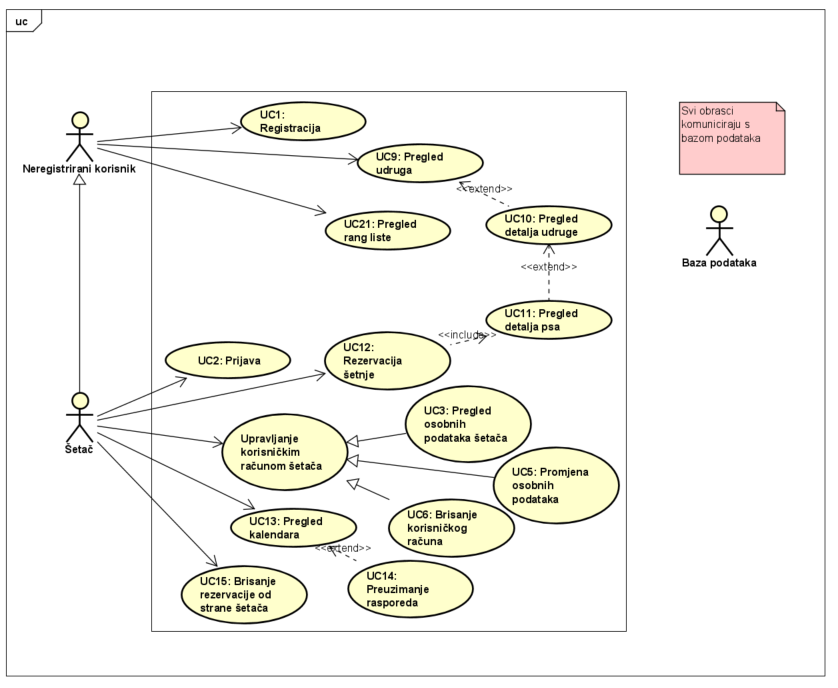
\includegraphics[scale=0.9]{dijagrami/uc-dijagram-1.PNG} 
	                	\centering
	                   	\caption{Dijagram obrasca uporabe, funkcionalnost neregistriranog korisnika i šetača}
	                	\label{fig:uc-1}
	                \end{figure}
	                
	                \begin{figure}[H]
		                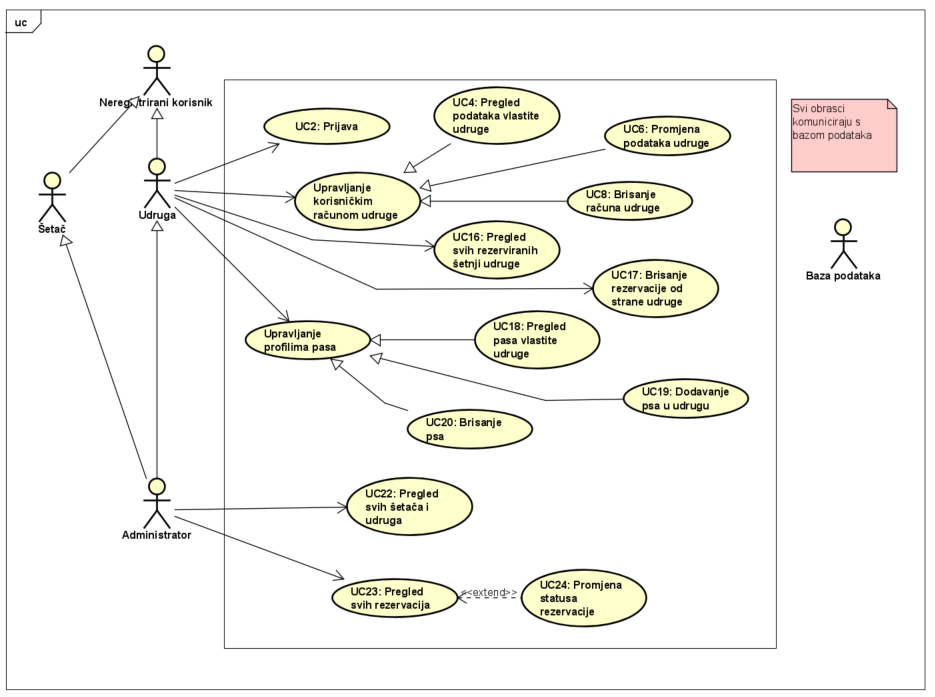
\includegraphics[scale=0.9]{dijagrami/uc-dijagram-2.PNG} 
	                	\centering
	                   	\caption{Dijagram obrasca uporabe, funkcionalnost udruge i administratora}
	                	\label{fig:uc-1}
	                \end{figure}
	                
				\eject		
				
			\subsection{Sekvencijski dijagrami}
				
				\noindent \textbf{Obrazac uporabe UC1 - Registracija}\\
				Korisnik bira opciju za registraciju šetača ili udruge te šalje zahtjev za registraciju. Poslužitelj prikazuje formu za odabranu registraciju. Korisnik unosi potrebne korisničke podatke. Poslužitelj provjerava ispravnost unesenih podataka i ako su valjani, u bazu podataka sprema podatke novog korisnika i obavještava ga o uspješnoj registraciji. Ako su elektronička pošta, korisničko ime ili formati nedozvoljeni, korisnika se obavještava o neuspješnoj registraciji i vraća na stranicu za registraciju.
				
				\begin{figure}[H]
					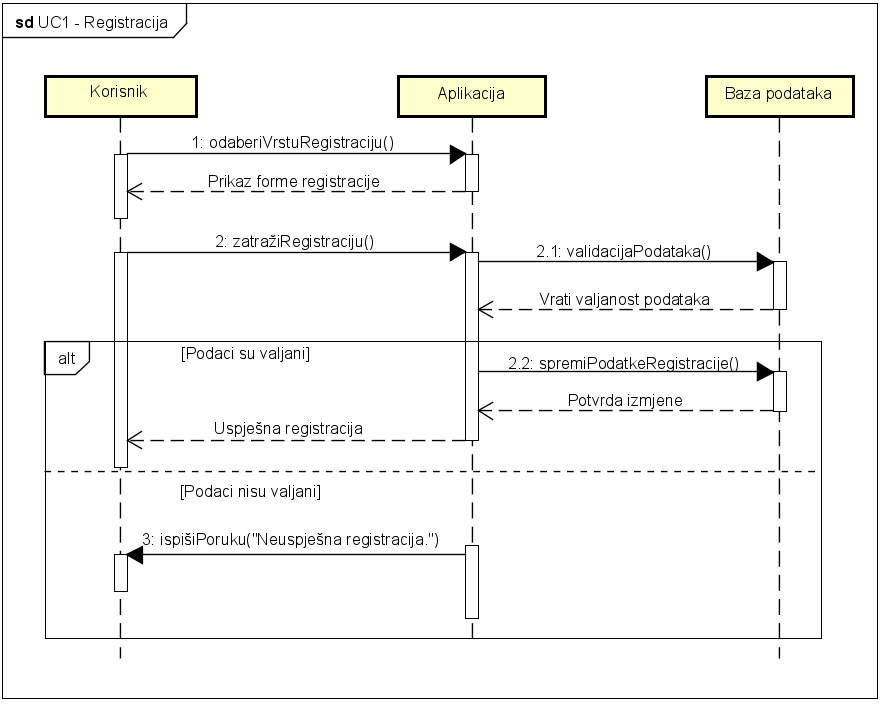
\includegraphics[scale=0.7]{dijagrami/UC1-Registracija.PNG} 
					\centering
					\caption{Sekvencijski dijagram za registraciju korisnika}
					\label{fig:uc-1}
				\end{figure}
				
				\eject
				
				\noindent \textbf{Obrazac uporabe UC5 - Promjena osobnih podataka}\\
				Korisnik bira opciju “Promijeni osobne podatke”. Poslužitelj vraća formu za unos novih podataka. Korisnik potom unosi nove podatke i potvrđuje promjenu. Poslužitelj provjerava valjanost novih podataka preko baze podataka. Ako su podaci valjani, poslužitelj šalje podatke korisnika u bazu podataka kako bi se stare vrijednosti ažurirale. Baza podataka vraća potvrdu poslužitelju koja šalje poruku o uspješnoj promijeni. U suprotnom, korisnika se obavještava o neuspješnoj promjeni podataka.
				
				\begin{figure}[H]
					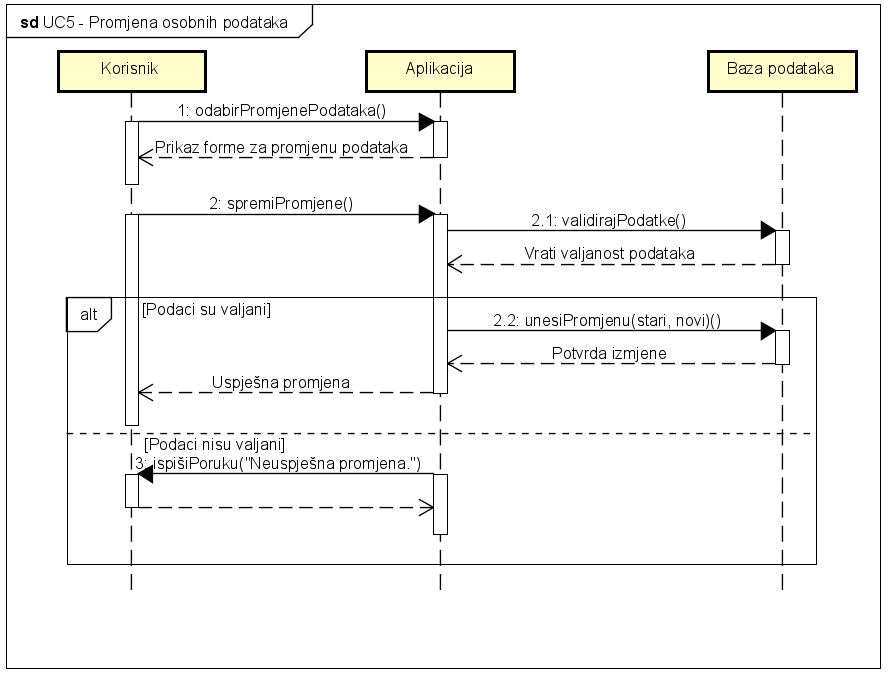
\includegraphics[scale=0.7]{dijagrami/UC5-Promjena-osobnih-podataka.PNG} 
					\centering
					\caption{Sekvencijski dijagram za promjenu osobnih podataka korisnika}
					\label{fig:uc-1}
				\end{figure}
				
				\eject
				
				\noindent \textbf{Obrazac uporabe UC12 - Rezervacija šetnje}\\
				Korisnik bira opciju “Odaberi psa.”. Ako korisnik nije registriran, sustav navodi korisnika na stranicu za registraciju. Poslužitelj korisniku vraća opciju za rezervaciju pasa. Korisnik bira određenog psa na što poslužitelj prikazuje njegovu raspoloživost te nudi opciju rezervacije. Korisnik bira termin na što mu poslužitelj vraća prikaz odabira i opciju grupne šetnje. Korisnik potvrđuje svoj odabir ako se odluči za individualnu šetnju. Odabirom opcije grupne šetnje poslužitelj iz baze dohvaća dostupne pse iz iste udruge u odabranom terminu i prikazuje korisniku. Korisnik bira pse za grupnu šetnju i potvrđuje svoj odabir, nakon čega poslužitelj dodaje novu rezervaciju u bazu koja vraća poruku potvrde i obavještava korisnika o uspješnoj rezervaciji.
				
				\begin{figure}[H]
					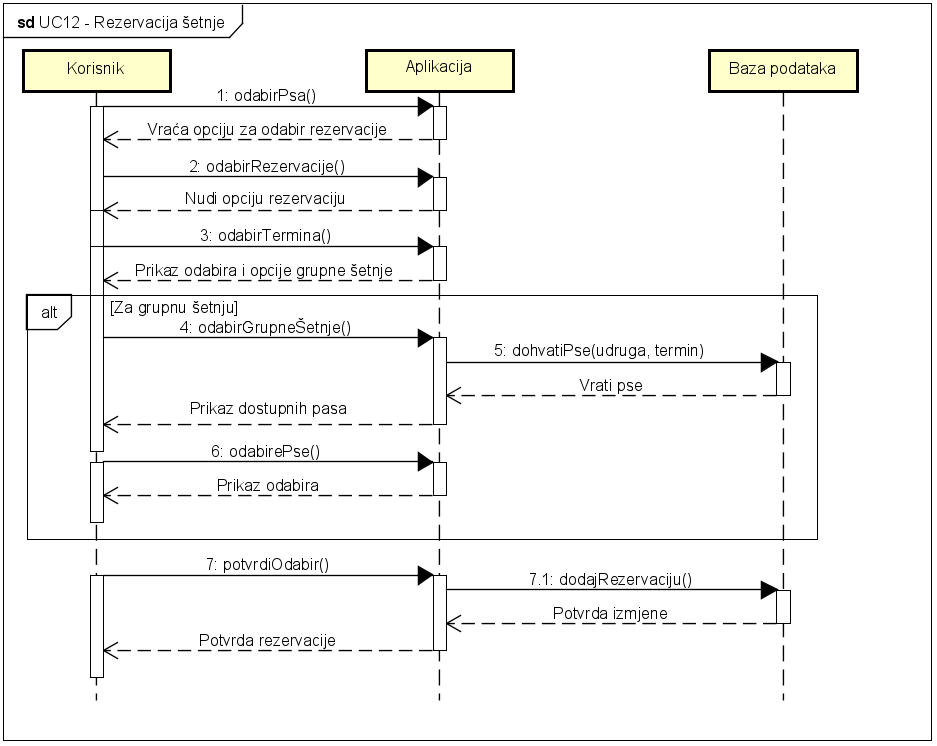
\includegraphics[scale=0.7]{dijagrami/UC12-Rezervacija-setnje.PNG} 
					\centering
					\caption{Sekvencijski dijagram za rezerviranje šetnji}
					\label{fig:uc-1}
				\end{figure}
				
				\eject
				
				
				
		\section{Ostali zahtjevi}
		
		    
		    \begin{packed_item}
		        \item Sustav treba biti implementiran kao web-aplikacija koristeći objektno orijentiranu paradigmu
		        \item Sustav treba omogućiti rad više korisnika u stvarnom vremenu
		        \item Sustav treba podržavati funkcionalnosti neovisno o vrsti uređaja, preglednika ili veličini ekrana
		        \item Nadogradnja sustava ne smije narušavati postojeće funkcionalnosti sustava
		        \item Veza s bazom podataka mora biti kvalitetno zaštićena, brza i otporna na vanjske greške
		        \item Izvršavanje dijela programa u kojem se pristupa bazi podataka ne smije trajati dulje od nekoliko sekundi
		        \item Korisnički podaci trebaju biti sigurno pohranjeni i odgovarajuće enkriptirani
		        \item Pristup sustavu mora biti omogućen iz javne mreže
		        \item Korisničko sučelje treba biti jednostavno, intuitivno i pregledno, korisnici se moraju znati koristiti sučeljem bez opširnih uputa
		        \item Neispravno korištenje korisničkog sučelja ne smije narušiti funkcionalnost i rad sustava
		        \item Korisničko sučelje i sustav moraju podržavati hrvatsku abecedu (dijakritičke znakove) pri unosu i prikazu tekstualnog sadržaja
		        \item Sustav treba koristiti odgovarajući europski format datuma (\textit{DD.MM.YYYY.})
		        
		    \end{packed_item}
		    
	